\documentclass{article}
\usepackage{hyperref}
\usepackage{graphicx}
%\usepackage{algorithmicx}
\usepackage{algorithm2e}

\begin{document}

\title{Resequencing against a variation graph}

\author{Erik Garrison}

\maketitle

\begin{abstract}
Despite the availability of whole genome sequences from many individuals in many species, when examining a new genome we only use single reference genome as our basis for interpretation.
As a result, our analyses are biased against the detection of any variation comprising significant differences from our reference.
Furthermore, in many contexts we may not have a completely linearized reference genome, and could avoid the need to collapse our reference into a series of small contigs for resequencing by directly resequencing against a high-quality assembly graph.
To answer these needs, we explore the use of sequence graphs that simultaneously describe many genomes.
We first describe a variety of models that can have been used to solve the problem in particular contexts.
We then outline a general, unrestricted model for sequence variation graphs that describes the common ground between these approaches.
Finally, we develop a practical implementation of this model and apply it to the construction of a sequence graph representing the whole genomes of 2500 individuals.
\end{abstract}

\section{Introduction}

Where genomes are small and sequences from different individuals can be reliably isolated, we can understand variation by assembling whole genomes and then comparing them via whole-genome comparison approaches \cite{mummer}.
In practice, complete genomes are rare, and we require prior information to reduce the cost of our efforts.
The genomes of organisms of interest (such as \emph{Homo sapiens}) are often large \cite{pmid11237011}, and would be costly to work with this way.
Or, they may simply be difficult to completely assemble reliably using existing technology (for example, the current reference for \emph{Plasmodium falciparum} still contains 80 gaps \cite{pfalciparum, pfalciparumweb}).

To enable genomics without requiring expensive full \emph{de novo} assemblies of each new sample, we localize short, cheap reads against a single high-quality reference genome.
While expedient, this approach biases our results towards a reference that may poorly-represent alleles present in the sample we are attempting to characterize.
We would like to align to a genome that is as similar to our sample as possible, ideally a ``personalized'' reference genome \cite{Yuan_2012}.

One way to achieve this would be to align against a reference system that contains known common variation from related individuals of the same species.
Such a system could take a number of forms, and to motivate our particular solution we first review different approaches to representing many sequences in the same context.
%Then, we develop and evaluate a generic software framework that can enable the construction and alignment to different kinds of sequence graphs.

\subsection{Issues with resequencing against a linear reference}

In \emph{resequencing}, we use alignments against a set of reference sequences (typically chromosomes or assembly contigs) to describe variation in a new sample.
By linking new observations into a common reference system, resequencing provides a coherent approach to relate the genomes of individuals in an entire population.
This approach requires sufficient similarity between variant sequences in order to relate them.
As a result, we may be unable to directly observe sequences which diverge significantly from the reference, such as large insertions and deletions of sequence (indels) or even clusters of smaller variation (such as single nucleotide polymorphisms, SNPs).
Indels, which contribute significantly to sequence diversity \cite{mills2010}, present a particular difficulty, in that sequences derived from insertions relative to the reference sequence cannot be easily localized against the reference.
This contributes significantly to the complexity of genotyping transposable element insertion polymorphisms, which are still poorly-understood despite the efforts of large-scale sequencing projects \cite{stewart2011}.
Similarly, copy-number variations, which influence large regions of the human genome, are difficult to genotype in new samples even when previously-known \cite{sudmant2010}.
%Resources such as that produced by the 1000 Genomes Project now contain the vast majority (greater than $95\%$) of variation that we expect to find in a newly-sequenced human individual \cite{1000Gphase1}.
%If we could generate a reference system including this variation, we could reduce the cost of genotyping it in new samples.

\begin{figure}[t]
\centering
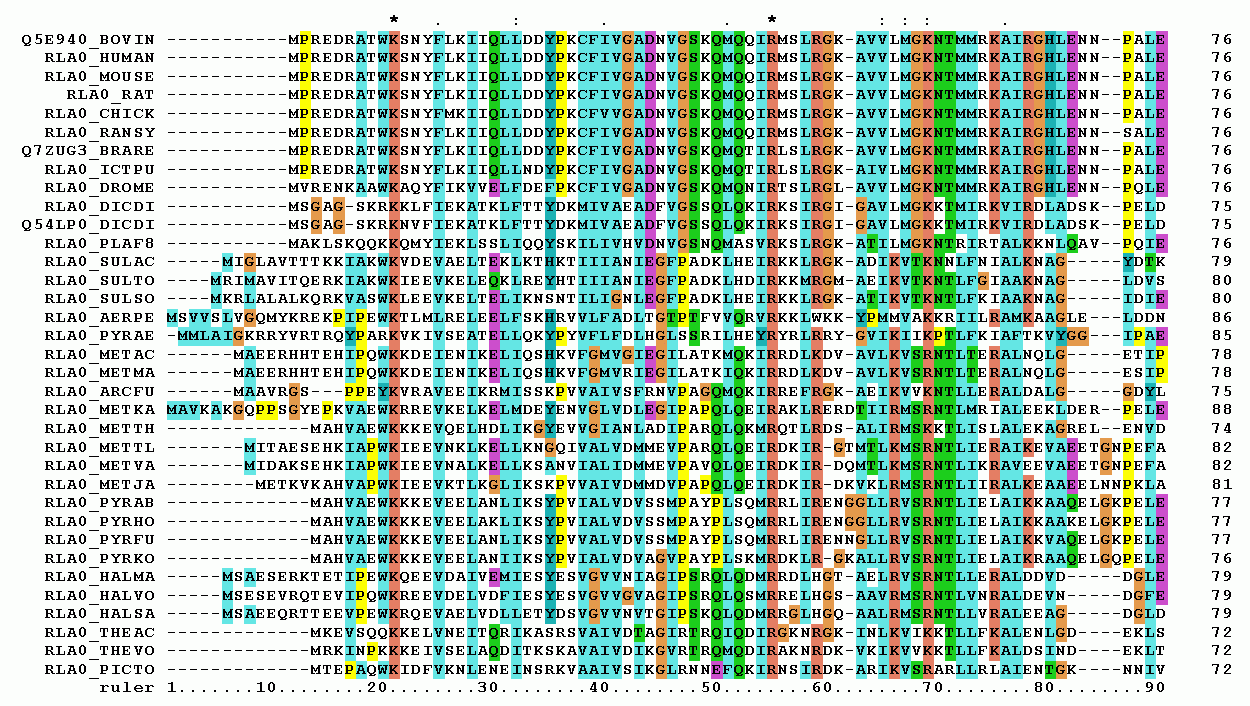
\includegraphics[width=1.0\textwidth]{figures/RPLP0_90_ClustalW_aln}
\caption{\label{fig:msa}
  First 90 positions of a protein multiple sequence alignment of instances of the acidic ribosomal protein P0 (L10E) from several organisms. Generated with ClustalX. Credit: Miguel Andrade \url{https://commons.wikimedia.org/wiki/File:RPLP0_90_ClustalW_aln.gif}. CC BY-SA 3.0.
}
\end{figure}

\subsection{Partially-ordered sequence graphs}

A common model used to combine variation from many samples into one reference system is a multiple sequence alignment (MSA, figure \ref{fig:msa}). In this approach, sequences are encoded using an additional gap character, typically represented as ``-'', which indicates when one sequence in the MSA has additional sequence where the one in which the gap is included does not. This mutually-gapped alignment has the desirable property that it fully-represents all of the sequences which were mutually aligned. This model has a dual representation as a partially-ordered graph in which nodes contain sequences in the alphabet of allowed characters (A, C, G, T for DNA, or the amino acids codes for proteins). In this partially-ordered graph, homologous aligned sequences are compressed into a single node or series of nodes (figure \ref{fig:poa}). Generalizations of pairwise alignment \cite{gotoh1982} allow the alignment of new sequences directly to this structure in $O(NM)$ time, where $N$ is the length of the query and $M$ the sum of lengths of unique sequences in the partially-ordered sequence graph \cite{lee2002POA}.

\begin{figure}[t]
\centering
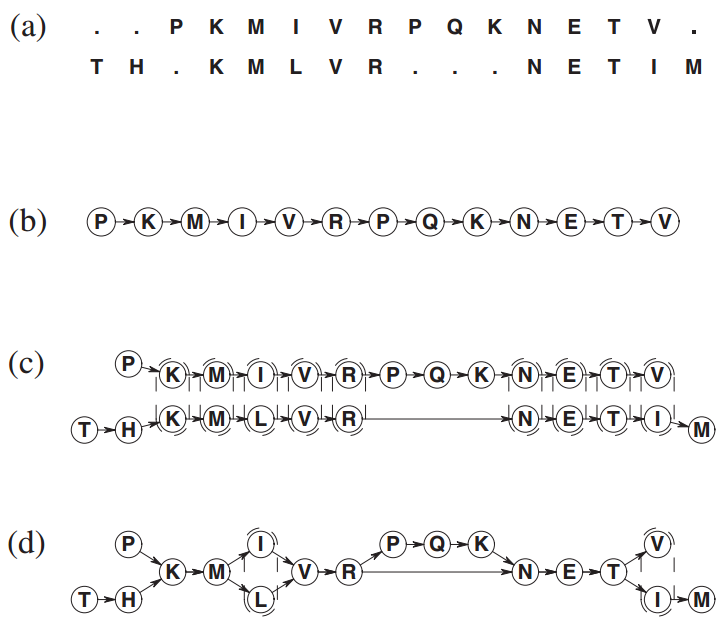
\includegraphics[width=0.8\textwidth]{figures/poamsa}
\caption{\label{fig:poa}
The relationship between a multiple sequence alignment (MSA) and a partially-ordered sequence graph (POA). (a) A gapped MSA representation for a pairwise protein alignment. (b) A single sequence in POA format. (c) The alignment of two sequences in POA format. (d) The POA representation of the original MSA. From \cite{lee2002POA}.
}
\end{figure}


\begin{figure}[t]
\centering
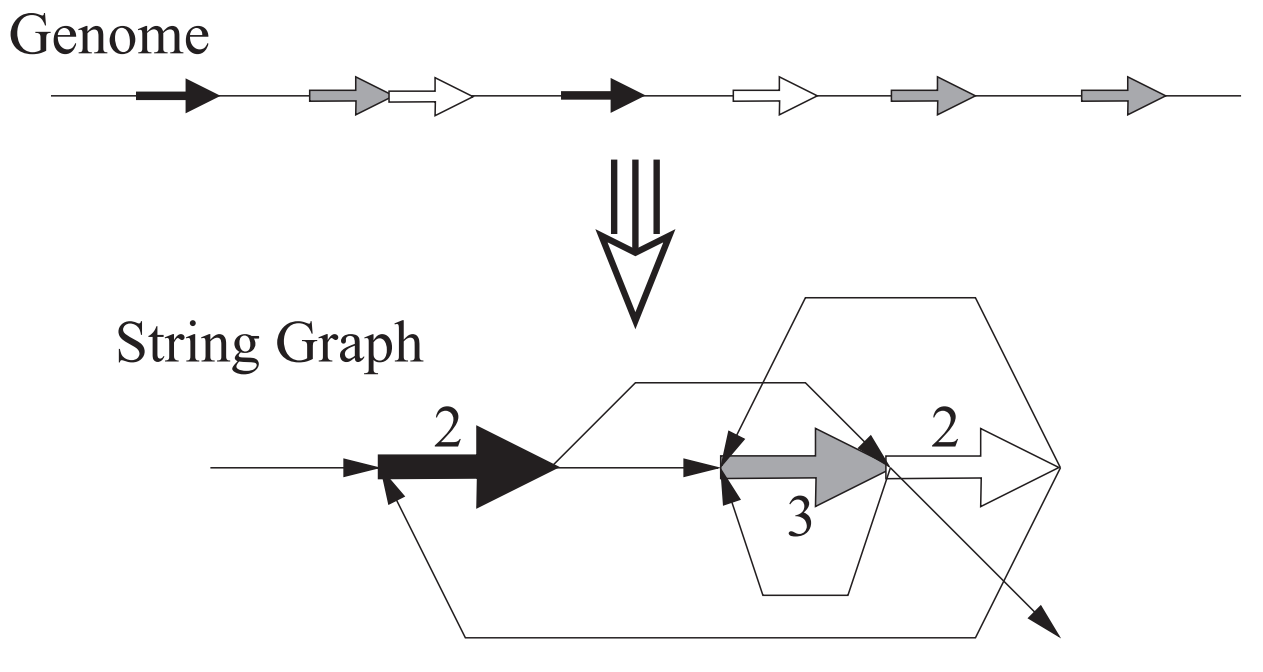
\includegraphics[width=1.0\textwidth]{figures/stringgraph}
\caption{\label{fig:stringgraph}
A genome and its string graph. Thick arrows illustrate identical, repeated sequences. Numbers describe copy-number counts. Edges represent linkages observed in shotgun sequencing data from the genome. From \cite{myers2005}.
}
\end{figure}

\subsection{Assemblies using string graphs and de Bruijn graphs}

While the partially-ordered representation of sequence variation can provide full information of many related sequences in a single model, the requirement of partial ordering limits its use to contexts where the complete synteny of a particular region can be established. A more general model for representing many sequences in the same context and allowing for cycles is the string graph, which was proposed by \cite{myers2005} and implemented efficiently at scale by \cite{simpson2010} in the SGA assembler. This represention captures and compresses all information about a genome or collection of genomes that can be derived from shotgun sequencing results (figure \ref{fig:stringgraph}). Sequences which are repeated in the input, such as transposons or copy number amplifications, are compressed into a single node in the string graph. The string graph does not require order, but this does not mean we could not use it as the basis for resequencing, as generalizations of string-to-graph alignment (e.g. POA) allow alignment of cyclic graphs to cyclic graphs \cite{myers1989}.

A similar approach to representing the sequences in a shotgun sequencing experiment in the same context is the de Bruijn graph. In this structure, each node represents a sequence of fixed size (a $k$-mer), and edges occur between nodes where the relationship $n_i[1, k] = n_j[0, k-1]$ is satisfied (note that $x[i, j]$ is a substring of $x$ from position $i$ to $j$). This structure has certain advantages conceptually over string graphs, in that it is often easier to operate on fixed-size kmers. However, as each novel $k$-mer in the graph will generate a series of new nodes, de Bruijn graph methods maintain reasonable memory usage by pruning low-abundance $k$-mers from the graph \cite{iqbal2012}. The lossy nature of practical implementations of this structure makes it less-attractive as a target model for representing many samples at the same time.

\subsection{Reference genome structures}

Recent work \cite{paten2014mapping} describes a comprehensive system that is related in scope to both string graphs and partially-ordered sequence graphs. In this \emph{reference genome structure}, sequences are attached to nodes and linkages between sequences occur where two sequences were observed in synteny in some haplotype in a reference set. This structure extends on other forms of sequence graphs by adding a mapping operation to the graph. In this \emph{left-right mapping} operation, the mapping of a new sequence (or more generally, another graph) into the existing reference system is driven by the discovery of unique contexts of a given length surrounding each node or neighborhood in the graph.

\subsection{Variation graphs}

In this effort, we sought to develop a practical implementation of a reference system that can (1) be used to represent and describe variation in many related samples (such as from the same species), (2) allow mapping of new sequences into this space, and (3) enable the genotyping (effectively copy-number assignment) of segments in the graph in a given individual or set of individuals whose sequencing results have been mapped into the system.

These requirements may be met by a number of underlying representations, but for the sake of expediency, we have chosen to implement first a generic model which places no restrictions on the structure of the graph. For instance, we do not require that repeated sequences are represented only once (as in string graphs), or that mappings require particularly-sized globally-unique contexts (as in reference genome structures). Nor is there a particular limit placed on the size of nodes. In a global context we allow for cycles, but when mapping we require the graph is partially ordered. This \emph{variation graph} is simply a general, assumption-free model that allows us to begin building a practical system to enable resequencing against both genome assemblies (e.g. string graphs) and partial orders such as are implied by a reference genome and a list of SNPs and indels.

\section{Methods}

\subsection{Model}

Formally, our model is a graph $G = ( N, E )$ comprised of a set of nodes $N = n_1 \ldots n_M$ and a set of directed edges $E = e_1 \ldots e_L$ such that $|N| = M$ and $|E| = L$. Each node $n_i$ represents a sequence $seq(n_i)$ which is built from an arbitrary alphabet $l$.
For DNA sequences, we might use $l = \{ A, T, G, C, N \}$, but in principle the model can be based in any alphabet.
Edges represent linkages between sequences that have been observed in a reference set of samples or other sequences. We identify edges by the pairs of node ids that they conect: $e_{i \rightarrow j} = \{ i, j \}$.
An edge $e_{i \rightarrow j}$ from $i$ to $j$ indicates that we have observed some sequence $n_i + n_j$.

\begin{figure}[t]
\centering
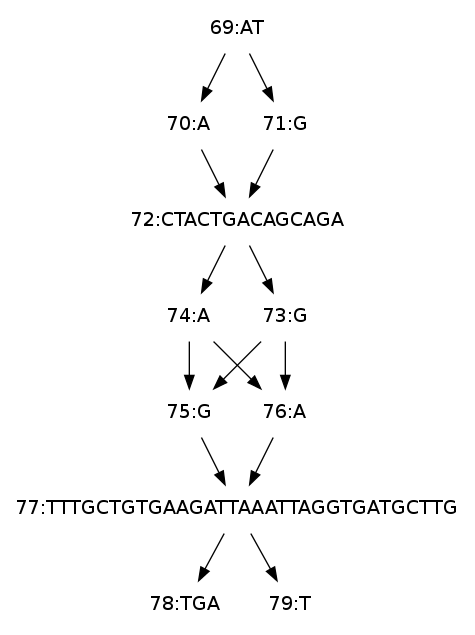
\includegraphics[width=0.6\textwidth]{figures/variationgraph}
\caption{\label{fig:variationgraph}
A fragment of a larger variation graph derived from simulated genomes. Nodes are labeled by their id and their sequence.
}
\end{figure}

\subsection{Interchange format and library implementation}

Experience with VCF \cite{danecek2011} and BAM \cite{li2009sambam} suggested that process of generating binary file formats is inimical to the productivity of scientific programmers.
So to implement our variant graph format we used an increasingly-standard approach, and implemented the format as a schema which is then compiled into a software implementation by a specialized compiler. (In our case, we used protocol buffers \cite{protobuf}, but a number of similar methods exist.)
We complied the schema (\url{https://github.com/ekg/vg/blob/master/vg.proto}) into a C++ library which can be used to manipulate the basic entities in the graph (nodes and edges) and secondary descriptions of them, such as sequence alignments.
The resulting library defines a set of classes representing our graph whose in-memory and on-wire (or on-disk) representation is nearly identical.
This allows us to efficiently store and retrieve fragments of the graph in a database, without incurring significantly more overhead than if the graph fragments were simple strings.

We extend the basic classes produced by the protocol buffer compiler by wrapping them in a convenience class (VG) which defines a number of abstract operations on the graph. This graph object forms the core of a local alignment algorithm, a disk-based indexing system, and a mapper that employs both these modules to align reads against a large graph using $k$-mer matching and local partial-order alignment. These functions are exposed by the command-line utility \emph{vg} (\url{https://github.com/ekg/vg}), which provides the following interface:

\begin{description}  \itemsep1pt \parskip0pt \parsep0pt
  \item[ construct    ] graph construction
  \item[ view         ] conversion (protobuf/json/GFA)
  \item[ index        ] index features of the graph in a disk-backed key/value store
  \item[ find         ] use an index to find nodes, edges, kmers, or positions
  \item[ paths        ] traverse paths in the graph
  \item[ align        ] local alignment
  \item[ map          ] global alignment
  \item[ stats        ] metrics describing graph properties
  \item[ join         ] combine graphs via a new head
  \item[ ids          ] manipulate node ids
  \item[ concat       ] concatenate graphs tail-to-head
\end{description}

\begin{figure}[t]
\centering
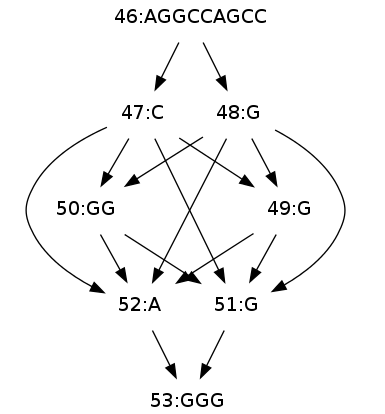
\includegraphics[width=0.5\textwidth]{figures/complexjunction}
\caption{\label{fig:complexjunction}
  An illustration of a complex portion of a variation graph. This represents a C/G SNP, followed immediately by a reference-relative insertion of a G, then an A/G SNP.
}
\end{figure}

\begin{function}[h!]
  \label{func:cut}
  $i \gets 0$ \\
  $j \gets 0$ \\
  \While{$i < position(d)$}{
      $i \gets i + |seq(n_j)|$ \\
      $j \gets j + 1$ \\
  }
  $l \gets position(d) - (i - |seq(n_j)|)$ \\
  $h \gets i$ \\
  $k \gets j$ \\
  \While{$h < position(d) + l$}{
      $h \gets i + |seq(n_k)|$ \\
      $k \gets k + 1$ \\
  }
  $r \gets position(d) - (h - |seq(n_k)|)$ \\
  $left \gets n_j[0, l]$ \\
  \If{$length(d) > 0$}{
    $middle \gets n_j[l, |n_j|]\ldots n_k[0, r]$
  }
  $right \gets n_k[r+length(d), |n_k|]$ \\
  \Return $n_0\ldots n_j-1, left, middle, right, n_k+1\ldots n_{|w|}$ \\
  \caption{Cut($w$, $d$) cuts path $w$ as defined by difference $d$}
\end{function}

\begin{algorithm}[h!]
  $R \gets $ reference sequence \\
  $G \gets ( R, \emptyset )$ \\
  \For{$d \in$ input}{
    $R \gets Cut(R, d)$ \\
    $n_l \gets $ node to the left of the cut \\
    $n_m \gets $ node in the middle of the cut (or $null$ if none exists) \\
    $n_r \gets $ node to the right of the cut \\
    \If{$length(d) > 0$}{
      add $e_{n_r \rightarrow n_l}$ to $G$
    }
    \If{$|seq(d)| > 0$}{
      add $n_a \gets seq(d)$ to $G$ \\
      add path $right,n,left$ to $G$ \\
      \For{$\forall n \notin R : \exists e_{n \rightarrow n_m} \lor \exists e_{n \rightarrow n_r}$}{
        add $e_{n \rightarrow n_a}$ to $G$
      }
    }
  }
  \caption{
\label{alg:construct}
Graph construction from a list of variants and a reference}
\end{algorithm}



\subsection{Graph construction}

As most population-scale data is available in VCF format, we have developed a construction method that takes a VCF file and FASTA reference genome as input and produces a variant graph (VG) data stream as output.
The algorithm can be executed in parallel for chunks of regions of the genome. For efficiency on multi-processor systems, we implemented a parallel algorithm based on OpenMP compiler directives.

Each variant represents a difference $d_i = { n, p, l, s }$, where $n$ is a node, $p$ is a position, $l$ is a length, and $s$ is a new string which replaces $l$ positions in $n$ to form a new node $n'$.
Let our our graph be a single node $R = n_r$ representing the reference.
Now, instead of creating a new sequence such that $|n| = |R|$ for each variant, we can cut $R$ at $p$ and $p+l$, creating 2 nodes when $l = 0$ (as in insertions) or 3 nodes when $l > 0$.
This cut operation yields a graph that has more nodes and edges, but represents exatly the same set of sequences.
To construct a graph from a VCF file we extend this cut operation to paths, which we represent as lists of nodes $w = n_0 \ldots n_{|w|}$:

In algorithm \ref{alg:construct}, we iteratively apply this cut function to the reference path to generate a graph based on the variants. To incorporate our variation into the growing graph, we (1) create new nodes for novel sequences, (2) link nodes in the reference path to span deletions, and (3) create edges connecting these nodes into the existing graph. The result is a directed acyclic graph that is equivalent to a multiple sequence alignment (a PO-MSA).

The algorithm is relatively straightforward, but we must take care to connect non-reference nodes together when they occur at successive reference positions. This can lead to relatively complex structures, as shown in figure \ref{fig:complexjunction}


\begin{function}[h!]
  \label{func:kpaths+}
  $children \gets \forall n' : \exists e_{n' \rightarrow n} \in G$ \\
  $w \gets \emptyset$ \\
  \eIf{$children = \emptyset$}{
    add $p$ to $w$
  }{
    \For{$c$ in $children$}{
      \eIf{$|seq(c)| < k$}{
        add kpaths+($c$, $p$, $w$, $k-|seq(c)|$, $G$) to $w$
      }{
        $p' \gets p + c$ \\
        $w \gets w + p'$
      }
    }
  }
  \Return $w$
  \caption{kpaths+($n$, $p$, $k$, $G$) generates paths prefixed by $p$ that extend \emph{right} no more than $k$ from node $n$ }
\end{function}

\begin{function}[h!]
  \label{func:kpaths-}
  $parents \gets \forall n' : \exists e_{n \rightarrow n'} \in G$ \\
  $w \gets \emptyset$ \\
  \eIf{$parents = \emptyset$}{
    add $s$ to $w$
  }{
    \For{$p$ in $parents$}{
      \eIf{$|seq(p)| < k$}{
        add kpaths-($p$, $p$, $w$, $k-|seq(p)|$, $G$) to $w$
      }{
        $s' \gets p + s$ \\
        $w \gets w + s'$
      }
    }
  }
  \Return $w$
  \caption{kpaths-($n$, $s$, $k$, $G$) generates paths suffixed by $s$ that extend \emph{left} no more than $k$ from node $n$ }
\end{function}

\begin{function}[h!]
  \label{func:kpaths}
  $emptyp \gets []$ \\
  $prev \gets $kpaths-($n$, $emptyp$, $k$, $G$) \\
  $next \gets $kpaths+($n$, $emptyp$, $k$, $G$) \\
  \Return $prev \cap next$ 
  \caption{kpaths($n$, $k$, $G$) generates paths that extend from $n$ no more than $k$ letters }
\end{function}

\begin{algorithm}[h!]
  $I$ is our index \\
  $k$ is our target $k$-mer size \\
  \For{$n \in G$}{
    \For{$w \in $ kpaths($n$, $k$, $G$)}{
      \For{$k \in $ $k$-mers of $w$}{
        $I[k] \gets $ ids of nodes in $w$
      }
    }
  }
  \caption{
\label{alg:kpaths}
Generate $k-$paths of a graph
}
\end{algorithm}


\subsection{Indexing}

A reference sequence is much-less useful if we can't quickly find subsequences matching a particular pattern in it. Here we describe the design of an indexing system that supports mapping reads into the variation graph.

An ideal indexing strategy would allow the query of sequences of any length directly from the index, a property which is typified by suffix arrays \cite{puglisi2007taxonomy}. Compressed suffix arrays exploit redundancies in the indexed corpus to reduce their memory usage. In the context of linear sequences, the relationship between the compressible Burrows-Wheeler transform and the suffix array has been used to generate very memory-efficient alignment algorithms \cite{li2013aligning}. Extensions of this model extend the underlying sequence to be a directed acyclic graph, but existing implementations have only provided this at a high (100X) cost in runtime \cite{siren2011indexing, huang2013short} relative to indexes based on linear sequences.

A simple, if less memory-efficient approach is to index $k$-mers of a particular size corresponding to positions (or nodes) within the reference (or graph), as is done in popular query tools such as blat \cite{kent2002blat} and short-read aligners like Mosaik \cite{lee2014mosaik} and Novoalign (\url{http://novocraft.com}).
Sequences can then be queried by breaking them into their components $k$-mers, looking these up, and clustering the results using the positional information provided in the index.
``Local'' alignment can then be used to refine the description of the mapping between the query and the reference.

In our context, we have an additional problem. Whereas we can easily obtain subsequences from a linear reference, obtaining the sequence of a particular node from our graph requires us to load the entire system into memory. We could include a serialized index in our interchange format, but this would add complexity to a simple specification.

To index the variant graph, first we implement a graph database using a disk-backed key value store. We use key namespacing to generate tables, and maintain interleaved tables for nodes and edges. Our values are serialized graph objects (nodes and edges). We can now add $k$-mer based keys to this graph, where the values are sets of nodes and positions in these nodes where the particular $k$-mers are found.

Indexing is straightforward provided the set of all paths of the graph, which would contain the set of $k$-mers that we'd like to index over. Problematically, the set of all paths of the graph is very large, on the order of $|G|^{|G|}$. But, as we are only interested in paths of a given length, we can bound the problem by working from $k-$paths, which we define as paths that extend no more than $k$ letters beyond a given (arbitrary) node.

We first define two recursive, depth-first searches to generate $k-$paths to the left (kpaths-) and right (kpaths+) of a given node. We then define a function which combines both of these to generate the $k-$paths for a given node (kpaths).
Finally, we combine these in an algorithm \ref{alg:kpaths} that iterates over the nodes in our graph and $k$-mers in their $k-$paths.


\begin{algorithm}[h!]
  $I \gets $ index of $G$ \\
  $k \gets $ $k$-mer size \\
  $q \gets $ query sequence \\
  graph $g \gets ( \emptyset, \emptyset )$ \\
  \For{$s \in kmers\_of(q, k)$}{
    extend $g$ with the $kmer\_subgraph(s \in I)$
  }
  our max-subgraph size $z \gets $ 0 \\
  \While{$z < |q|$}{
    $g \gets g + neighbors\_of\_nodes(g)$ \\
    $z \gets $ maximum length of a disjoint subgraph of $g$ \\
  }
  extend $g$ by joining its head nodes to a new, empty root node \\
  align $q$ to $g$ using POA \\
  \caption{
    \label{alg:map}
    Map a sequence $q$ to the graph
  }
\end{algorithm}


\subsection{Alignment}

Given a small graph, we can use partial order alignment (POA) \cite{lee2002POA} to generate an alignment between a novel sequence and our variation graph. To enable high-performance POA, we have followed the ``striped'' Smith-Waterman-Gotoh algorithm first described by \cite{farrar2007striped} as implemented in \cite{zhao2013ssw}, and adapted it to operate on partially-ordered sequence graphs to yield a parallel POA algorithm.

As genome-scale graphs will be very large, we cannot apply this algorithm to obtain optimal alignments. A standard alignment approach is to subset the reference system to regions that are likely to be similar to our target. Provided the $k$-mer index produced in the previous section, we can establish such regions by looking for the $k$-mers of our query sequence (given by the function $kmers\_of$) in the index, then building up a set of candidate neighborhoods in the graph and aligning to them.

Each $k$-mer $s$ corresponds to a subgraph $g$ of $G$ whose paths contain $s$. We call the function that returns this subgraph $kmer\_subgraph$. Each graph may contain several disjoint subgraphs $g_1\ldots g_x$, such that $g_i \cup g_j = \emptyset \forall i \ne j \in [0,x]$. If we query the index for the graph neighborhoods which contain paths matching our $s$, we can expect not to be able to align $s$ until one of the subgraphs has paths that are at least as large as $s$.

We thus construct a simple read mapping algorithm \ref{alg:map} by obtaining a $k$-mer subgraph $g$ for $s$, and expanding its neighborhood incrementally by adding neighbor nodes until the maximum subgraph size is at least $|s|$. Once this criteria is met, we have a good chance of being able to obtain an full alignment of our sequence to the graph. Local alignment can be obtained by joining the subgraphs of $g$ to a single root node, and then aligning against this structure in one pass using POA. The resulting alignment describes an optimal path through a set of nodes as well as novel differences between the sequence and the aligned nodes in the variation graph. Provided the ids used for the nodes are maintained through alignment, the alignment can be contextualized into the full graph despite being defined against a dynamically-constructed subgraph.


\section{Results}

\subsection{Tests of the command-line API}

The command-line API provided by $vg$ is validated through a series of tests which can be run by executing ``make test'' in the project repository. These include evaluations of graph construction, conversion into other formats, local alignment, mapping (alignment using an index), index generation and querying (find), id manipulation, graph concatenation, and the generation of statistics describing variation graphs. See \url{https://github.com/ekg/vg/tree/master/test/t} for the corresponding examples.

\subsection{Construction of a variation graph from 2500 individuals}

We apply $vg$ to the construction of a reference graph for the \href{http://www.1000genomes.org/announcements/phase3-variant-calls-chry-are-available-variant-calls-chrx-have-been-updated-2014-11-0}{1000 Genomes Phase 3 release}, which includes more than 80 million sequence variants across 2500 individuals. This process took approximately 24 hours on a 48-core AMD Opteron system (@ 2.8GHz). Construction times varyied due to other use of the system during this process, but ran from approximately 100 CPU hours for larger chromosomes (1,2,3) to 10 CPU hours for smaller ones (20,21,22). For exposition, we used ``vg stats'' to generate statistics about the size of the variation graph for each chromosome \ref{tab:1000G}. The total on-disk size of the graphs is 11 gigabytes, which is 2.6 times the size of the un-annotated variants in the VCF file (position, reference, alternate = 1.3G) plus the reference (3.0G).
% ? what is the amount of added sequence in the graph relative to the reference?
% borked... doh

\begin{table}[h!]
\begin{tabular}{ r || r | r | r | r | r | r }
chrom & nodes & edges & length & megabytes & bp/node & bp/edge \\
\hline
1 & 18807182 & 25672337 & 255749560 & 692.448 & 13.5985 & 9.96207 \\
2 & 20596983 & 28111941 & 250307338 & 730.599 & 12.1526 & 8.90395 \\
3 & 16964872 & 23148775 & 203879166 & 598.185 & 12.0177 & 8.80734 \\
4 & 16662385 & 22748535 & 196908702 & 584.318 & 11.8176 & 8.65588 \\
5 & 15312827 & 20898032 & 186201209 & 541.313 & 12.1598 & 8.90999 \\
6 & 14596378 & 19934148 & 176166408 & 514.529 & 12.0692 & 8.83742 \\
7 & 13707313 & 18722684 & 163876860 & 481.261 & 11.9554 & 8.75285 \\
8 & 13370034 & 18268435 & 150983815 & 460.811 & 11.2927 & 8.26474 \\
9 & 10355399 & 14140342 & 144791971 & 381.707 & 13.9823 & 10.2396 \\
10 & 11595435 & 15848168 & 139550146 & 406.938 & 12.0349 & 8.80544 \\
11 & 11760220 & 16063146 & 139073676 & 410.37 & 11.8258 & 8.65794 \\
12 & 11239089 & 15348804 & 137742373 & 396.459 & 12.2557 & 8.97414 \\
13 & 8304286 & 11334524 & 118039004 & 306.398 & 14.2142 & 10.4141 \\
14 & 7714325 & 10536695 & 110018123 & 284.534 & 14.2615 & 10.4414 \\
15 & 7045525 & 9623586 & 104966483 & 263.49 & 14.8983 & 10.9072 \\
16 & 7837318 & 10727847 & 93071991 & 271.556 & 11.8755 & 8.67574 \\
17 & 6757656 & 9242823 & 83542990 & 236.209 & 12.3627 & 9.03869 \\
18 & 6592027 & 8999627 & 80356045 & 228.961 & 12.1899 & 8.92882 \\
19 & 5305871 & 7273405 & 60979705 & 179.594 & 11.4929 & 8.38393 \\
20 & 5267910 & 7198915 & 64852993 & 182.151 & 12.311 & 9.00872 \\
21 & 3207033 & 4386537 & 49243049 & 117.292 & 15.3547 & 11.226 \\
22 & 3197025 & 4381733 & 52422299 & 120.171 & 16.3972 & 11.9638 \\
X & 10022133 & 13697203 & 158750551 & 387.294 & 15.84 & 11.59 \\
\end{tabular}

\caption{
Variation graphs generated from the 1000 Genomes final release, along with the number of basepairs per node and edge, to demonstrate average density of variation. The lengths of the chromosomes correspond to the total sequence in all samples in the project.
}
\label{tab:1000G}

\end{table}

\section{Discussion}

Here we have described a foundational system for the manipulation of a pan-genomic representation which we term a \emph{variation graph}. This system provides basic features that would be required if we were to engage in resequencing directly against this structure. We develop a binary interchange format for variation graphs and alignments against them. This format has a parallel representation in an on-disk index that allows fast querying of particular nodes and graph neighborhoods. We develop a method to index the $k$-mers of the variation graph and then align new sequences into the graph using this index to generate seeds.

Unfortunately, the available time for this work was limited, and we have not been able to explore several aspects of this problem, such as alignment against large graphs and genotyping or copy-number determination. The specific form which this process might follow is unclear. One can imagine that the process of ``variant calling'' might be replaced in this context by a graph pruning operation, in which candidate (sometimes novel) nodes in a graph describing all the sequencing result for a particular sample are removed where there is insufficient or inconsistent information. Other problems, such as how to communicate results derived entirely within this format to researchers who are accustomed to using a linear map of the genome, remain outside the immediate scope of this work.


%\pagebreak

\bibliography{references}{}

\bibliographystyle{plain}




\end{document}
